\documentclass[1p]{elsarticle_modified}
%\bibliographystyle{elsarticle-num}

%\usepackage[colorlinks]{hyperref}
%\usepackage{abbrmath_seonhwa} %\Abb, \Ascr, \Acal ,\Abf, \Afrak
\usepackage{amsfonts}
\usepackage{amssymb}
\usepackage{amsmath}
\usepackage{amsthm}
\usepackage{scalefnt}
\usepackage{amsbsy}
\usepackage{kotex}
\usepackage{caption}
\usepackage{subfig}
\usepackage{color}
\usepackage{graphicx}
\usepackage{xcolor} %% white, black, red, green, blue, cyan, magenta, yellow
\usepackage{float}
\usepackage{setspace}
\usepackage{hyperref}

\usepackage{tikz}
\usetikzlibrary{arrows}

\usepackage{multirow}
\usepackage{array} % fixed length table
\usepackage{hhline}

%%%%%%%%%%%%%%%%%%%%%
\makeatletter
\renewcommand*\env@matrix[1][\arraystretch]{%
	\edef\arraystretch{#1}%
	\hskip -\arraycolsep
	\let\@ifnextchar\new@ifnextchar
	\array{*\c@MaxMatrixCols c}}
\makeatother %https://tex.stackexchange.com/questions/14071/how-can-i-increase-the-line-spacing-in-a-matrix
%%%%%%%%%%%%%%%

\usepackage[normalem]{ulem}

\newcommand{\msout}[1]{\ifmmode\text{\sout{\ensuremath{#1}}}\else\sout{#1}\fi}
%SOURCE: \msout is \stkout macro in https://tex.stackexchange.com/questions/20609/strikeout-in-math-mode

\newcommand{\cancel}[1]{
	\ifmmode
	{\color{red}\msout{#1}}
	\else
	{\color{red}\sout{#1}}
	\fi
}

\newcommand{\add}[1]{
	{\color{blue}\uwave{#1}}
}

\newcommand{\replace}[2]{
	\ifmmode
	{\color{red}\msout{#1}}{\color{blue}\uwave{#2}}
	\else
	{\color{red}\sout{#1}}{\color{blue}\uwave{#2}}
	\fi
}

\newcommand{\Sol}{\mathcal{S}} %segment
\newcommand{\D}{D} %diagram
\newcommand{\A}{\mathcal{A}} %arc


%%%%%%%%%%%%%%%%%%%%%%%%%%%%%5 test

\def\sl{\operatorname{\textup{SL}}(2,\Cbb)}
\def\psl{\operatorname{\textup{PSL}}(2,\Cbb)}
\def\quan{\mkern 1mu \triangleright \mkern 1mu}

\theoremstyle{definition}
\newtheorem{thm}{Theorem}[section]
\newtheorem{prop}[thm]{Proposition}
\newtheorem{lem}[thm]{Lemma}
\newtheorem{ques}[thm]{Question}
\newtheorem{cor}[thm]{Corollary}
\newtheorem{defn}[thm]{Definition}
\newtheorem{exam}[thm]{Example}
\newtheorem{rmk}[thm]{Remark}
\newtheorem{alg}[thm]{Algorithm}

\newcommand{\I}{\sqrt{-1}}
\begin{document}

%\begin{frontmatter}
%
%\title{Boundary parabolic representations of knots up to 8 crossings}
%
%%% Group authors per affiliation:
%\author{Yunhi Cho} 
%\address{Department of Mathematics, University of Seoul, Seoul, Korea}
%\ead{yhcho@uos.ac.kr}
%
%
%\author{Seonhwa Kim} %\fnref{s_kim}}
%\address{Center for Geometry and Physics, Institute for Basic Science, Pohang, 37673, Korea}
%\ead{ryeona17@ibs.re.kr}
%
%\author{Hyuk Kim}
%\address{Department of Mathematical Sciences, Seoul National University, Seoul 08826, Korea}
%\ead{hyukkim@snu.ac.kr}
%
%\author{Seokbeom Yoon}
%\address{Department of Mathematical Sciences, Seoul National University, Seoul, 08826,  Korea}
%\ead{sbyoon15@snu.ac.kr}
%
%\begin{abstract}
%We find all boundary parabolic representation of knots up to 8 crossings.
%
%\end{abstract}
%\begin{keyword}
%    \MSC[2010] 57M25 
%\end{keyword}
%
%\end{frontmatter}

%\linenumbers
%\tableofcontents
%
\newcommand\colored[1]{\textcolor{white}{\rule[-0.35ex]{0.8em}{1.4ex}}\kern-0.8em\color{red} #1}%
%\newcommand\colored[1]{\textcolor{white}{ #1}\kern-2.17ex	\textcolor{white}{ #1}\kern-1.81ex	\textcolor{white}{ #1}\kern-2.15ex\color{red}#1	}

{\Large $\underline{11a_{252}~(K11a_{252})}$}

\setlength{\tabcolsep}{10pt}
\renewcommand{\arraystretch}{1.6}
\vspace{1cm}\begin{tabular}{m{100pt}>{\centering\arraybackslash}m{274pt}}
\multirow{5}{120pt}{
	\centering
	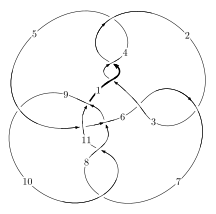
\includegraphics[width=112pt]{../../../GIT/diagram.site/Diagrams/png/501_11a_252.png}\\
\ \ \ A knot diagram\footnotemark}&
\allowdisplaybreaks
\textbf{Linearized knot diagam} \\
\cline{2-2}
 &
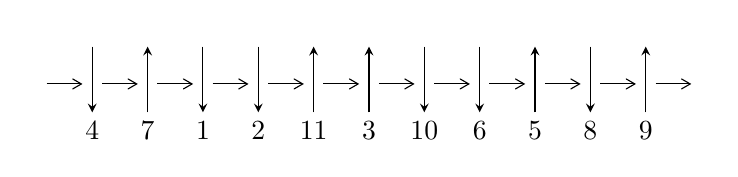
\begin{tikzpicture}[x=20pt, y=17pt]
	% nodes
	\node (C0) at (0, 0) {};
	\node (C1) at (1, 0) {};
	\node (C1U) at (1, +1) {};
	\node (C1D) at (1, -1) {4};

	\node (C2) at (2, 0) {};
	\node (C2U) at (2, +1) {};
	\node (C2D) at (2, -1) {7};

	\node (C3) at (3, 0) {};
	\node (C3U) at (3, +1) {};
	\node (C3D) at (3, -1) {1};

	\node (C4) at (4, 0) {};
	\node (C4U) at (4, +1) {};
	\node (C4D) at (4, -1) {2};

	\node (C5) at (5, 0) {};
	\node (C5U) at (5, +1) {};
	\node (C5D) at (5, -1) {11};

	\node (C6) at (6, 0) {};
	\node (C6U) at (6, +1) {};
	\node (C6D) at (6, -1) {3};

	\node (C7) at (7, 0) {};
	\node (C7U) at (7, +1) {};
	\node (C7D) at (7, -1) {10};

	\node (C8) at (8, 0) {};
	\node (C8U) at (8, +1) {};
	\node (C8D) at (8, -1) {6};

	\node (C9) at (9, 0) {};
	\node (C9U) at (9, +1) {};
	\node (C9D) at (9, -1) {5};

	\node (C10) at (10, 0) {};
	\node (C10U) at (10, +1) {};
	\node (C10D) at (10, -1) {8};

	\node (C11) at (11, 0) {};
	\node (C11U) at (11, +1) {};
	\node (C11D) at (11, -1) {9};
	\node (C12) at (12, 0) {};

	% arrows
	\draw[->,>={angle 60}]
	(C0) edge (C1) (C1) edge (C2) (C2) edge (C3) (C3) edge (C4) (C4) edge (C5) (C5) edge (C6) (C6) edge (C7) (C7) edge (C8) (C8) edge (C9) (C9) edge (C10) (C10) edge (C11) (C11) edge (C12) ;	\draw[->,>=stealth]
	(C1U) edge (C1D) (C2D) edge (C2U) (C3U) edge (C3D) (C4U) edge (C4D) (C5D) edge (C5U) (C6D) edge (C6U) (C7U) edge (C7D) (C8U) edge (C8D) (C9D) edge (C9U) (C10U) edge (C10D) (C11D) edge (C11U) ;
	\end{tikzpicture} \\
\hhline{~~} \\& 
\textbf{Solving Sequence} \\ \cline{2-2} 
 &
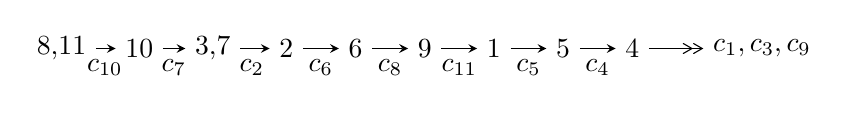
\begin{tikzpicture}[x=25pt, y=7pt]
	% node
	\node (A0) at (-1/8, 0) {8,11};
	\node (A1) at (1, 0) {10};
	\node (A2) at (33/16, 0) {3,7};
	\node (A3) at (25/8, 0) {2};
	\node (A4) at (33/8, 0) {6};
	\node (A5) at (41/8, 0) {9};
	\node (A6) at (49/8, 0) {1};
	\node (A7) at (57/8, 0) {5};
	\node (A8) at (65/8, 0) {4};
	\node (C1) at (1/2, -1) {$c_{10}$};
	\node (C2) at (3/2, -1) {$c_{7}$};
	\node (C3) at (21/8, -1) {$c_{2}$};
	\node (C4) at (29/8, -1) {$c_{6}$};
	\node (C5) at (37/8, -1) {$c_{8}$};
	\node (C6) at (45/8, -1) {$c_{11}$};
	\node (C7) at (53/8, -1) {$c_{5}$};
	\node (C8) at (61/8, -1) {$c_{4}$};
	\node (A9) at (10, 0) {$c_{1},c_{3},c_{9}$};

	% edge
	\draw[->,>=stealth]	
	(A0) edge (A1) (A1) edge (A2) (A2) edge (A3) (A3) edge (A4) (A4) edge (A5) (A5) edge (A6) (A6) edge (A7) (A7) edge (A8) ;
	\draw[->>,>={angle 60}]	
	(A8) edge (A9);
\end{tikzpicture} \\ 

\end{tabular} \\

\footnotetext{
The image of knot diagram is generated by the software ``\textbf{Draw programme}" developed by Andrew Bartholomew(\url{http://www.layer8.co.uk/maths/draw/index.htm\#Running-draw}), where we modified some parts for our purpose(\url{https://github.com/CATsTAILs/LinksPainter}).
}\phantom \\ \newline 
\centering \textbf{Ideals for irreducible components\footnotemark of $X_{\text{par}}$} 
 
\begin{align*}
I^u_{1}&=\langle 
-4.11167\times10^{157} u^{70}+9.80349\times10^{157} u^{69}+\cdots+6.48947\times10^{158} b+1.66763\times10^{158},\\
\phantom{I^u_{1}}&\phantom{= \langle  }3.33659\times10^{158} u^{70}-7.80024\times10^{158} u^{69}+\cdots+6.48947\times10^{158} a+4.59343\times10^{159},\;u^{71}-2 u^{70}+\cdots+10 u+1\rangle \\
I^u_{2}&=\langle 
- u^3+u^2+b-1,\;- u^5+u^4- u^2+a+u-1,\;u^6- u^5- u^4+2 u^3- u+1\rangle \\
\\
\end{align*}
\raggedright * 2 irreducible components of $\dim_{\mathbb{C}}=0$, with total 77 representations.\\
\footnotetext{All coefficients of polynomials are rational numbers. But the coefficients are sometimes approximated in decimal forms when there is not enough margin.}
\newpage
\renewcommand{\arraystretch}{1}
\centering \section*{I. $I^u_{1}= \langle -4.11\times10^{157} u^{70}+9.80\times10^{157} u^{69}+\cdots+6.49\times10^{158} b+1.67\times10^{158},\;3.34\times10^{158} u^{70}-7.80\times10^{158} u^{69}+\cdots+6.49\times10^{158} a+4.59\times10^{159},\;u^{71}-2 u^{70}+\cdots+10 u+1 \rangle$}
\flushleft \textbf{(i) Arc colorings}\\
\begin{tabular}{m{7pt} m{180pt} m{7pt} m{180pt} }
\flushright $a_{8}=$&$\begin{pmatrix}0\\u\end{pmatrix}$ \\
\flushright $a_{11}=$&$\begin{pmatrix}1\\0\end{pmatrix}$ \\
\flushright $a_{10}=$&$\begin{pmatrix}1\\- u^2\end{pmatrix}$ \\
\flushright $a_{3}=$&$\begin{pmatrix}-0.514154 u^{70}+1.20198 u^{69}+\cdots-14.4737 u-7.07828\\0.0633591 u^{70}-0.151068 u^{69}+\cdots+3.49569 u-0.256975\end{pmatrix}$ \\
\flushright $a_{7}=$&$\begin{pmatrix}u\\- u^3+u\end{pmatrix}$ \\
\flushright $a_{2}=$&$\begin{pmatrix}-0.573953 u^{70}+1.19350 u^{69}+\cdots-13.1744 u-7.01032\\0.0951502 u^{70}-0.228949 u^{69}+\cdots+3.45444 u-0.317091\end{pmatrix}$ \\
\flushright $a_{6}=$&$\begin{pmatrix}0.174897 u^{70}-0.472490 u^{69}+\cdots+15.3667 u+5.67523\\-0.118550 u^{70}+0.321518 u^{69}+\cdots-1.35288 u+0.169544\end{pmatrix}$ \\
\flushright $a_{9}=$&$\begin{pmatrix}-0.337748 u^{70}+0.603848 u^{69}+\cdots-25.8435 u+0.618193\\-0.177165 u^{70}+0.217073 u^{69}+\cdots-2.82251 u-0.449303\end{pmatrix}$ \\
\flushright $a_{1}=$&$\begin{pmatrix}0.0798159 u^{70}-0.254371 u^{69}+\cdots+8.28970 u+3.25294\\u^3- u\end{pmatrix}$ \\
\flushright $a_{5}=$&$\begin{pmatrix}0.293446 u^{70}-0.794009 u^{69}+\cdots+16.7196 u+5.50568\\-0.118550 u^{70}+0.321518 u^{69}+\cdots-1.35288 u+0.169544\end{pmatrix}$ \\
\flushright $a_{4}=$&$\begin{pmatrix}-0.360696 u^{70}+0.644610 u^{69}+\cdots-4.30465 u-3.28034\\0.0395576 u^{70}-0.0960173 u^{69}+\cdots+2.98896 u-0.198923\end{pmatrix}$\\ \flushright $a_{4}=$&$\begin{pmatrix}-0.360696 u^{70}+0.644610 u^{69}+\cdots-4.30465 u-3.28034\\0.0395576 u^{70}-0.0960173 u^{69}+\cdots+2.98896 u-0.198923\end{pmatrix}$\\&\end{tabular}
\flushleft \textbf{(ii) Obstruction class $= -1$}\\~\\
\flushleft \textbf{(iii) Cusp Shapes $= 3.60654 u^{70}-6.89818 u^{69}+\cdots-6.61880 u-2.95587$}\\~\\
\newpage\renewcommand{\arraystretch}{1}
\flushleft \textbf{(iv) u-Polynomials at the component}\newline \\
\begin{tabular}{m{50pt}|m{274pt}}
Crossings & \hspace{64pt}u-Polynomials at each crossing \\
\hline $$\begin{aligned}c_{1},c_{3},c_{4}\end{aligned}$$&$\begin{aligned}
&u^{71}-7 u^{70}+\cdots-3 u+1
\end{aligned}$\\
\hline $$\begin{aligned}c_{2},c_{6}\end{aligned}$$&$\begin{aligned}
&u^{71}- u^{70}+\cdots+320 u+64
\end{aligned}$\\
\hline $$\begin{aligned}c_{5}\end{aligned}$$&$\begin{aligned}
&u^{71}+6 u^{70}+\cdots+2 u+1
\end{aligned}$\\
\hline $$\begin{aligned}c_{7},c_{10}\end{aligned}$$&$\begin{aligned}
&u^{71}-2 u^{70}+\cdots+10 u+1
\end{aligned}$\\
\hline $$\begin{aligned}c_{8}\end{aligned}$$&$\begin{aligned}
&u^{71}-6 u^{70}+\cdots-3424 u+319
\end{aligned}$\\
\hline $$\begin{aligned}c_{9}\end{aligned}$$&$\begin{aligned}
&u^{71}-2 u^{70}+\cdots+35022 u+3953
\end{aligned}$\\
\hline $$\begin{aligned}c_{11}\end{aligned}$$&$\begin{aligned}
&u^{71}+12 u^{70}+\cdots-2 u-1
\end{aligned}$\\
\hline
\end{tabular}\\~\\
\newpage\renewcommand{\arraystretch}{1}
\flushleft \textbf{(v) Riley Polynomials at the component}\newline \\
\begin{tabular}{m{50pt}|m{274pt}}
Crossings & \hspace{64pt}Riley Polynomials at each crossing \\
\hline $$\begin{aligned}c_{1},c_{3},c_{4}\end{aligned}$$&$\begin{aligned}
&y^{71}-67 y^{70}+\cdots-45 y-1
\end{aligned}$\\
\hline $$\begin{aligned}c_{2},c_{6}\end{aligned}$$&$\begin{aligned}
&y^{71}+39 y^{70}+\cdots-36864 y-4096
\end{aligned}$\\
\hline $$\begin{aligned}c_{5}\end{aligned}$$&$\begin{aligned}
&y^{71}+12 y^{70}+\cdots-6 y-1
\end{aligned}$\\
\hline $$\begin{aligned}c_{7},c_{10}\end{aligned}$$&$\begin{aligned}
&y^{71}-48 y^{70}+\cdots-10 y-1
\end{aligned}$\\
\hline $$\begin{aligned}c_{8}\end{aligned}$$&$\begin{aligned}
&y^{71}-72 y^{70}+\cdots+3210942 y-101761
\end{aligned}$\\
\hline $$\begin{aligned}c_{9}\end{aligned}$$&$\begin{aligned}
&y^{71}-48 y^{70}+\cdots-314283574 y-15626209
\end{aligned}$\\
\hline $$\begin{aligned}c_{11}\end{aligned}$$&$\begin{aligned}
&y^{71}+72 y^{69}+\cdots-10 y-1
\end{aligned}$\\
\hline
\end{tabular}\\~\\
\newpage\flushleft \textbf{(vi) Complex Volumes and Cusp Shapes}
$$\begin{array}{c|c|c}  
\text{Solutions to }I^u_{1}& \I (\text{vol} + \sqrt{-1}CS) & \text{Cusp shape}\\
 \hline 
\begin{aligned}
u &= \phantom{-}0.973828 + 0.280461 I \\
a &= -0.382377 + 0.191990 I \\
b &= \phantom{-}0.806691 - 0.545143 I\end{aligned}
 & \phantom{-}0.16886 - 3.43064 I & \phantom{-0.000000 } 0 \\ \hline\begin{aligned}
u &= \phantom{-}0.973828 - 0.280461 I \\
a &= -0.382377 - 0.191990 I \\
b &= \phantom{-}0.806691 + 0.545143 I\end{aligned}
 & \phantom{-}0.16886 + 3.43064 I & \phantom{-0.000000 } 0 \\ \hline\begin{aligned}
u &= -1.039510 + 0.064875 I \\
a &= \phantom{-}1.72385 - 3.92841 I \\
b &= \phantom{-}0.153087 - 0.345660 I\end{aligned}
 & -2.19246 + 1.77118 I & \phantom{-0.000000 } 0 \\ \hline\begin{aligned}
u &= -1.039510 - 0.064875 I \\
a &= \phantom{-}1.72385 + 3.92841 I \\
b &= \phantom{-}0.153087 + 0.345660 I\end{aligned}
 & -2.19246 - 1.77118 I & \phantom{-0.000000 } 0 \\ \hline\begin{aligned}
u &= -1.04817\phantom{ +0.000000I} \\
a &= \phantom{-}2.58690\phantom{ +0.000000I} \\
b &= \phantom{-}0.574511\phantom{ +0.000000I}\end{aligned}
 & -4.26740\phantom{ +0.000000I} & \phantom{-}40.4800\phantom{ +0.000000I} \\ \hline\begin{aligned}
u &= -0.093891 + 1.051200 I \\
a &= \phantom{-}0.826346 - 0.088868 I \\
b &= \phantom{-}1.35016 - 0.97545 I\end{aligned}
 & -2.29132 + 4.25686 I & \phantom{-0.000000 } 0 \\ \hline\begin{aligned}
u &= -0.093891 - 1.051200 I \\
a &= \phantom{-}0.826346 + 0.088868 I \\
b &= \phantom{-}1.35016 + 0.97545 I\end{aligned}
 & -2.29132 - 4.25686 I & \phantom{-0.000000 } 0 \\ \hline\begin{aligned}
u &= -1.051030 + 0.111007 I \\
a &= -4.50600 - 1.44719 I \\
b &= \phantom{-}1.07671 - 1.20500 I\end{aligned}
 & -3.57140 + 0.57623 I & \phantom{-0.000000 } 0 \\ \hline\begin{aligned}
u &= -1.051030 - 0.111007 I \\
a &= -4.50600 + 1.44719 I \\
b &= \phantom{-}1.07671 + 1.20500 I\end{aligned}
 & -3.57140 - 0.57623 I & \phantom{-0.000000 } 0 \\ \hline\begin{aligned}
u &= \phantom{-}1.080020 + 0.152289 I \\
a &= -0.273682 - 1.001120 I \\
b &= \phantom{-}0.031630 - 1.096560 I\end{aligned}
 & -2.62165 - 3.78828 I & \phantom{-0.000000 } 0\\
 \hline 
 \end{array}$$\newpage$$\begin{array}{c|c|c}  
\text{Solutions to }I^u_{1}& \I (\text{vol} + \sqrt{-1}CS) & \text{Cusp shape}\\
 \hline 
\begin{aligned}
u &= \phantom{-}1.080020 - 0.152289 I \\
a &= -0.273682 + 1.001120 I \\
b &= \phantom{-}0.031630 + 1.096560 I\end{aligned}
 & -2.62165 + 3.78828 I & \phantom{-0.000000 } 0 \\ \hline\begin{aligned}
u &= \phantom{-}0.202728 + 0.884593 I \\
a &= -0.558547 - 0.125884 I \\
b &= -0.708883 + 0.771941 I\end{aligned}
 & \phantom{-}2.34440 + 1.95014 I & \phantom{-}4.45936 - 2.53493 I \\ \hline\begin{aligned}
u &= \phantom{-}0.202728 - 0.884593 I \\
a &= -0.558547 + 0.125884 I \\
b &= -0.708883 - 0.771941 I\end{aligned}
 & \phantom{-}2.34440 - 1.95014 I & \phantom{-}4.45936 + 2.53493 I \\ \hline\begin{aligned}
u &= -1.043640 + 0.390448 I \\
a &= -0.683454 + 0.373591 I \\
b &= \phantom{-}0.003299 - 0.591740 I\end{aligned}
 & -1.92491 + 1.08364 I & \phantom{-0.000000 } 0 \\ \hline\begin{aligned}
u &= -1.043640 - 0.390448 I \\
a &= -0.683454 - 0.373591 I \\
b &= \phantom{-}0.003299 + 0.591740 I\end{aligned}
 & -1.92491 - 1.08364 I & \phantom{-0.000000 } 0 \\ \hline\begin{aligned}
u &= \phantom{-}0.599075 + 0.942927 I \\
a &= \phantom{-}0.393955 - 0.081858 I \\
b &= -0.131439 - 1.112940 I\end{aligned}
 & -1.031500 + 0.354146 I & \phantom{-0.000000 } 0 \\ \hline\begin{aligned}
u &= \phantom{-}0.599075 - 0.942927 I \\
a &= \phantom{-}0.393955 + 0.081858 I \\
b &= -0.131439 + 1.112940 I\end{aligned}
 & -1.031500 - 0.354146 I & \phantom{-0.000000 } 0 \\ \hline\begin{aligned}
u &= \phantom{-}1.119810 + 0.032767 I \\
a &= \phantom{-}0.413302 - 0.046036 I \\
b &= -1.43154 - 0.47309 I\end{aligned}
 & -5.71064 - 0.88851 I & \phantom{-0.000000 } 0 \\ \hline\begin{aligned}
u &= \phantom{-}1.119810 - 0.032767 I \\
a &= \phantom{-}0.413302 + 0.046036 I \\
b &= -1.43154 + 0.47309 I\end{aligned}
 & -5.71064 + 0.88851 I & \phantom{-0.000000 } 0 \\ \hline\begin{aligned}
u &= \phantom{-}1.117600 + 0.093371 I \\
a &= \phantom{-}0.678615 - 0.967658 I \\
b &= -0.93853 - 1.07438 I\end{aligned}
 & -4.60632 - 2.57396 I & \phantom{-0.000000 } 0\\
 \hline 
 \end{array}$$\newpage$$\begin{array}{c|c|c}  
\text{Solutions to }I^u_{1}& \I (\text{vol} + \sqrt{-1}CS) & \text{Cusp shape}\\
 \hline 
\begin{aligned}
u &= \phantom{-}1.117600 - 0.093371 I \\
a &= \phantom{-}0.678615 + 0.967658 I \\
b &= -0.93853 + 1.07438 I\end{aligned}
 & -4.60632 + 2.57396 I & \phantom{-0.000000 } 0 \\ \hline\begin{aligned}
u &= -1.126210 + 0.132843 I \\
a &= -1.08363 + 2.70605 I \\
b &= -0.254130 + 0.145869 I\end{aligned}
 & -8.04028 + 4.80757 I & \phantom{-0.000000 } 0 \\ \hline\begin{aligned}
u &= -1.126210 - 0.132843 I \\
a &= -1.08363 - 2.70605 I \\
b &= -0.254130 - 0.145869 I\end{aligned}
 & -8.04028 - 4.80757 I & \phantom{-0.000000 } 0 \\ \hline\begin{aligned}
u &= -0.004277 + 1.135740 I \\
a &= \phantom{-}1.65575 + 0.09224 I \\
b &= \phantom{-}2.85653 + 0.65690 I\end{aligned}
 & \phantom{-}0.43763 + 6.35749 I & \phantom{-0.000000 } 0 \\ \hline\begin{aligned}
u &= -0.004277 - 1.135740 I \\
a &= \phantom{-}1.65575 - 0.09224 I \\
b &= \phantom{-}2.85653 - 0.65690 I\end{aligned}
 & \phantom{-}0.43763 - 6.35749 I & \phantom{-0.000000 } 0 \\ \hline\begin{aligned}
u &= -0.116710 + 0.856297 I \\
a &= -1.89294 + 0.32292 I \\
b &= -2.33201 - 0.18461 I\end{aligned}
 & -1.12559 + 1.87856 I & -4.53889 - 4.17402 I \\ \hline\begin{aligned}
u &= -0.116710 - 0.856297 I \\
a &= -1.89294 - 0.32292 I \\
b &= -2.33201 + 0.18461 I\end{aligned}
 & -1.12559 - 1.87856 I & -4.53889 + 4.17402 I \\ \hline\begin{aligned}
u &= \phantom{-}0.987158 + 0.647225 I \\
a &= -0.078094 - 0.228604 I \\
b &= -0.086973 + 0.620891 I\end{aligned}
 & -2.28261 - 6.08346 I & \phantom{-0.000000 } 0 \\ \hline\begin{aligned}
u &= \phantom{-}0.987158 - 0.647225 I \\
a &= -0.078094 + 0.228604 I \\
b &= -0.086973 - 0.620891 I\end{aligned}
 & -2.28261 + 6.08346 I & \phantom{-0.000000 } 0 \\ \hline\begin{aligned}
u &= -0.794072 + 0.043433 I \\
a &= -0.28211 + 1.87433 I \\
b &= -0.540687 - 0.121257 I\end{aligned}
 & -1.42339 + 1.14206 I & -7.64564 - 4.36852 I\\
 \hline 
 \end{array}$$\newpage$$\begin{array}{c|c|c}  
\text{Solutions to }I^u_{1}& \I (\text{vol} + \sqrt{-1}CS) & \text{Cusp shape}\\
 \hline 
\begin{aligned}
u &= -0.794072 - 0.043433 I \\
a &= -0.28211 - 1.87433 I \\
b &= -0.540687 + 0.121257 I\end{aligned}
 & -1.42339 - 1.14206 I & -7.64564 + 4.36852 I \\ \hline\begin{aligned}
u &= \phantom{-}1.192200 + 0.296593 I \\
a &= \phantom{-}0.317333 + 1.101890 I \\
b &= \phantom{-}0.334681 + 0.650646 I\end{aligned}
 & -8.79734 - 8.72585 I & \phantom{-0.000000 } 0 \\ \hline\begin{aligned}
u &= \phantom{-}1.192200 - 0.296593 I \\
a &= \phantom{-}0.317333 - 1.101890 I \\
b &= \phantom{-}0.334681 - 0.650646 I\end{aligned}
 & -8.79734 + 8.72585 I & \phantom{-0.000000 } 0 \\ \hline\begin{aligned}
u &= -0.670063 + 0.347596 I \\
a &= -0.08138 + 1.61220 I \\
b &= \phantom{-}0.355159 - 0.164091 I\end{aligned}
 & -6.99999 - 3.26565 I & -6.82531 + 6.65441 I \\ \hline\begin{aligned}
u &= -0.670063 - 0.347596 I \\
a &= -0.08138 - 1.61220 I \\
b &= \phantom{-}0.355159 + 0.164091 I\end{aligned}
 & -6.99999 + 3.26565 I & -6.82531 - 6.65441 I \\ \hline\begin{aligned}
u &= -0.645193 + 1.117580 I \\
a &= \phantom{-}1.213880 - 0.359050 I \\
b &= \phantom{-}1.77925 + 1.40756 I\end{aligned}
 & -7.91168 + 0.39314 I & \phantom{-0.000000 } 0 \\ \hline\begin{aligned}
u &= -0.645193 - 1.117580 I \\
a &= \phantom{-}1.213880 + 0.359050 I \\
b &= \phantom{-}1.77925 - 1.40756 I\end{aligned}
 & -7.91168 - 0.39314 I & \phantom{-0.000000 } 0 \\ \hline\begin{aligned}
u &= \phantom{-}1.200010 + 0.496938 I \\
a &= \phantom{-}0.218730 + 0.009510 I \\
b &= -0.699809 - 0.172100 I\end{aligned}
 & -0.76386 - 6.94431 I & \phantom{-0.000000 } 0 \\ \hline\begin{aligned}
u &= \phantom{-}1.200010 - 0.496938 I \\
a &= \phantom{-}0.218730 - 0.009510 I \\
b &= -0.699809 + 0.172100 I\end{aligned}
 & -0.76386 + 6.94431 I & \phantom{-0.000000 } 0 \\ \hline\begin{aligned}
u &= \phantom{-}0.003290 + 1.307520 I \\
a &= -1.45978 - 0.16433 I \\
b &= -2.98943 - 0.91001 I\end{aligned}
 & -5.26918 + 10.31530 I & \phantom{-0.000000 } 0\\
 \hline 
 \end{array}$$\newpage$$\begin{array}{c|c|c}  
\text{Solutions to }I^u_{1}& \I (\text{vol} + \sqrt{-1}CS) & \text{Cusp shape}\\
 \hline 
\begin{aligned}
u &= \phantom{-}0.003290 - 1.307520 I \\
a &= -1.45978 + 0.16433 I \\
b &= -2.98943 + 0.91001 I\end{aligned}
 & -5.26918 - 10.31530 I & \phantom{-0.000000 } 0 \\ \hline\begin{aligned}
u &= \phantom{-}0.452314 + 0.404120 I \\
a &= -0.369574 + 0.466412 I \\
b &= \phantom{-}0.728049 + 0.140839 I\end{aligned}
 & \phantom{-}1.57443 + 0.30385 I & \phantom{-}7.03884 + 0.55864 I \\ \hline\begin{aligned}
u &= \phantom{-}0.452314 - 0.404120 I \\
a &= -0.369574 - 0.466412 I \\
b &= \phantom{-}0.728049 - 0.140839 I\end{aligned}
 & \phantom{-}1.57443 - 0.30385 I & \phantom{-}7.03884 - 0.55864 I \\ \hline\begin{aligned}
u &= \phantom{-}1.328370 + 0.443679 I \\
a &= \phantom{-}0.18921 - 1.90014 I \\
b &= -2.43997 - 0.05463 I\end{aligned}
 & -5.52892 - 6.64078 I & \phantom{-0.000000 } 0 \\ \hline\begin{aligned}
u &= \phantom{-}1.328370 - 0.443679 I \\
a &= \phantom{-}0.18921 + 1.90014 I \\
b &= -2.43997 + 0.05463 I\end{aligned}
 & -5.52892 + 6.64078 I & \phantom{-0.000000 } 0 \\ \hline\begin{aligned}
u &= \phantom{-}1.41902 + 0.24540 I \\
a &= -0.31463 + 1.40902 I \\
b &= \phantom{-}1.50742 - 0.01617 I\end{aligned}
 & -14.7704 - 4.4090 I & \phantom{-0.000000 } 0 \\ \hline\begin{aligned}
u &= \phantom{-}1.41902 - 0.24540 I \\
a &= -0.31463 - 1.40902 I \\
b &= \phantom{-}1.50742 + 0.01617 I\end{aligned}
 & -14.7704 + 4.4090 I & \phantom{-0.000000 } 0 \\ \hline\begin{aligned}
u &= \phantom{-}1.36179 + 0.48894 I \\
a &= -0.271842 - 0.047925 I \\
b &= \phantom{-}1.037440 + 0.370809 I\end{aligned}
 & -6.81481 - 9.66907 I & \phantom{-0.000000 } 0 \\ \hline\begin{aligned}
u &= \phantom{-}1.36179 - 0.48894 I \\
a &= -0.271842 + 0.047925 I \\
b &= \phantom{-}1.037440 - 0.370809 I\end{aligned}
 & -6.81481 + 9.66907 I & \phantom{-0.000000 } 0 \\ \hline\begin{aligned}
u &= \phantom{-}1.36248 + 0.53740 I \\
a &= \phantom{-}0.15951 + 1.89725 I \\
b &= \phantom{-}2.64476 - 0.38758 I\end{aligned}
 & -3.85560 - 12.20440 I & \phantom{-0.000000 } 0\\
 \hline 
 \end{array}$$\newpage$$\begin{array}{c|c|c}  
\text{Solutions to }I^u_{1}& \I (\text{vol} + \sqrt{-1}CS) & \text{Cusp shape}\\
 \hline 
\begin{aligned}
u &= \phantom{-}1.36248 - 0.53740 I \\
a &= \phantom{-}0.15951 - 1.89725 I \\
b &= \phantom{-}2.64476 + 0.38758 I\end{aligned}
 & -3.85560 + 12.20440 I & \phantom{-0.000000 } 0 \\ \hline\begin{aligned}
u &= \phantom{-}0.019457 + 0.498656 I \\
a &= \phantom{-}2.06316 - 1.12594 I \\
b &= \phantom{-}0.125101 - 0.377825 I\end{aligned}
 & -5.36921 + 5.60292 I & -4.23205 - 1.95004 I \\ \hline\begin{aligned}
u &= \phantom{-}0.019457 - 0.498656 I \\
a &= \phantom{-}2.06316 + 1.12594 I \\
b &= \phantom{-}0.125101 + 0.377825 I\end{aligned}
 & -5.36921 - 5.60292 I & -4.23205 + 1.95004 I \\ \hline\begin{aligned}
u &= -1.35931 + 0.64552 I \\
a &= -0.08241 + 1.81423 I \\
b &= -3.25610 - 0.21443 I\end{aligned}
 & -4.09299 + 4.00272 I & \phantom{-0.000000 } 0 \\ \hline\begin{aligned}
u &= -1.35931 - 0.64552 I \\
a &= -0.08241 - 1.81423 I \\
b &= -3.25610 + 0.21443 I\end{aligned}
 & -4.09299 - 4.00272 I & \phantom{-0.000000 } 0 \\ \hline\begin{aligned}
u &= -1.45782 + 0.39176 I \\
a &= -0.64419 - 1.79501 I \\
b &= \phantom{-}2.93443 + 0.40813 I\end{aligned}
 & -4.54539 - 0.34097 I & \phantom{-0.000000 } 0 \\ \hline\begin{aligned}
u &= -1.45782 - 0.39176 I \\
a &= -0.64419 + 1.79501 I \\
b &= \phantom{-}2.93443 - 0.40813 I\end{aligned}
 & -4.54539 + 0.34097 I & \phantom{-0.000000 } 0 \\ \hline\begin{aligned}
u &= -1.42285 + 0.53580 I \\
a &= \phantom{-}0.953468 - 0.520457 I \\
b &= -0.57598 + 1.65551 I\end{aligned}
 & -6.35450 + 1.85292 I & \phantom{-0.000000 } 0 \\ \hline\begin{aligned}
u &= -1.42285 - 0.53580 I \\
a &= \phantom{-}0.953468 + 0.520457 I \\
b &= -0.57598 - 1.65551 I\end{aligned}
 & -6.35450 - 1.85292 I & \phantom{-0.000000 } 0 \\ \hline\begin{aligned}
u &= \phantom{-}1.41471 + 0.59221 I \\
a &= -0.31168 - 1.72898 I \\
b &= -2.57738 + 0.66185 I\end{aligned}
 & -9.7419 - 16.8559 I & \phantom{-0.000000 } 0\\
 \hline 
 \end{array}$$\newpage$$\begin{array}{c|c|c}  
\text{Solutions to }I^u_{1}& \I (\text{vol} + \sqrt{-1}CS) & \text{Cusp shape}\\
 \hline 
\begin{aligned}
u &= \phantom{-}1.41471 - 0.59221 I \\
a &= -0.31168 + 1.72898 I \\
b &= -2.57738 - 0.66185 I\end{aligned}
 & -9.7419 + 16.8559 I & \phantom{-0.000000 } 0 \\ \hline\begin{aligned}
u &= -0.230568 + 0.263555 I \\
a &= -2.27801 + 1.97060 I \\
b &= -0.913442 + 0.373094 I\end{aligned}
 & -1.31227 + 1.35935 I & -5.28068 - 4.63416 I \\ \hline\begin{aligned}
u &= -0.230568 - 0.263555 I \\
a &= -2.27801 - 1.97060 I \\
b &= -0.913442 - 0.373094 I\end{aligned}
 & -1.31227 - 1.35935 I & -5.28068 + 4.63416 I \\ \hline\begin{aligned}
u &= -1.45197 + 0.82397 I \\
a &= \phantom{-}0.15600 - 1.43654 I \\
b &= \phantom{-}3.48750 + 0.15031 I\end{aligned}
 & -10.25460 + 7.45224 I & \phantom{-0.000000 } 0 \\ \hline\begin{aligned}
u &= -1.45197 - 0.82397 I \\
a &= \phantom{-}0.15600 + 1.43654 I \\
b &= \phantom{-}3.48750 - 0.15031 I\end{aligned}
 & -10.25460 - 7.45224 I & \phantom{-0.000000 } 0 \\ \hline\begin{aligned}
u &= -1.71685 + 0.37143 I \\
a &= \phantom{-}0.56832 + 1.29788 I \\
b &= -3.07440 - 0.93374 I\end{aligned}
 & -11.03720 - 3.15602 I & \phantom{-0.000000 } 0 \\ \hline\begin{aligned}
u &= -1.71685 - 0.37143 I \\
a &= \phantom{-}0.56832 - 1.29788 I \\
b &= -3.07440 + 0.93374 I\end{aligned}
 & -11.03720 + 3.15602 I & \phantom{-0.000000 } 0 \\ \hline\begin{aligned}
u &= \phantom{-}0.039727 + 0.221588 I \\
a &= -3.96929 + 1.74892 I \\
b &= \phantom{-}0.178650 + 0.492128 I\end{aligned}
 & -0.04861 + 2.05474 I & -0.05845 - 2.58157 I \\ \hline\begin{aligned}
u &= \phantom{-}0.039727 - 0.221588 I \\
a &= -3.96929 - 1.74892 I \\
b &= \phantom{-}0.178650 - 0.492128 I\end{aligned}
 & -0.04861 - 2.05474 I & -0.05845 + 2.58157 I \\ \hline\begin{aligned}
u &= -0.125529 + 0.098090 I \\
a &= -5.80125 - 1.46490 I \\
b &= -0.727087 + 0.471790 I\end{aligned}
 & -2.61258 + 0.40782 I & -2.91513 + 1.25335 I\\
 \hline 
 \end{array}$$\newpage$$\begin{array}{c|c|c}  
\text{Solutions to }I^u_{1}& \I (\text{vol} + \sqrt{-1}CS) & \text{Cusp shape}\\
 \hline 
\begin{aligned}
u &= -0.125529 - 0.098090 I \\
a &= -5.80125 + 1.46490 I \\
b &= -0.727087 - 0.471790 I\end{aligned}
 & -2.61258 - 0.40782 I & -2.91513 - 1.25335 I\\
 \hline 
 \end{array}$$\newpage\newpage\renewcommand{\arraystretch}{1}
\centering \section*{II. $I^u_{2}= \langle - u^3+u^2+b-1,\;- u^5+u^4- u^2+a+u-1,\;u^6- u^5- u^4+2 u^3- u+1 \rangle$}
\flushleft \textbf{(i) Arc colorings}\\
\begin{tabular}{m{7pt} m{180pt} m{7pt} m{180pt} }
\flushright $a_{8}=$&$\begin{pmatrix}0\\u\end{pmatrix}$ \\
\flushright $a_{11}=$&$\begin{pmatrix}1\\0\end{pmatrix}$ \\
\flushright $a_{10}=$&$\begin{pmatrix}1\\- u^2\end{pmatrix}$ \\
\flushright $a_{3}=$&$\begin{pmatrix}u^5- u^4+u^2- u+1\\u^3- u^2+1\end{pmatrix}$ \\
\flushright $a_{7}=$&$\begin{pmatrix}u\\- u^3+u\end{pmatrix}$ \\
\flushright $a_{2}=$&$\begin{pmatrix}u^5- u^4+u^2- u+1\\u^3- u^2+1\end{pmatrix}$ \\
\flushright $a_{6}=$&$\begin{pmatrix}u\\- u^3+u\end{pmatrix}$ \\
\flushright $a_{9}=$&$\begin{pmatrix}- u^3\\u^5- u^3+u\end{pmatrix}$ \\
\flushright $a_{1}=$&$\begin{pmatrix}- u^3\\u^3- u\end{pmatrix}$ \\
\flushright $a_{5}=$&$\begin{pmatrix}u^3\\- u^3+u\end{pmatrix}$ \\
\flushright $a_{4}=$&$\begin{pmatrix}u^5- u^4+u^3+u^2- u+1\\- u^2+u+1\end{pmatrix}$\\ \flushright $a_{4}=$&$\begin{pmatrix}u^5- u^4+u^3+u^2- u+1\\- u^2+u+1\end{pmatrix}$\\&\end{tabular}
\flushleft \textbf{(ii) Obstruction class $= 1$}\\~\\
\flushleft \textbf{(iii) Cusp Shapes $= -3 u^5+7 u^4- u^3-6 u^2+5 u-1$}\\~\\
\newpage\renewcommand{\arraystretch}{1}
\flushleft \textbf{(iv) u-Polynomials at the component}\newline \\
\begin{tabular}{m{50pt}|m{274pt}}
Crossings & \hspace{64pt}u-Polynomials at each crossing \\
\hline $$\begin{aligned}c_{1}\end{aligned}$$&$\begin{aligned}
&(u-1)^6
\end{aligned}$\\
\hline $$\begin{aligned}c_{2},c_{6}\end{aligned}$$&$\begin{aligned}
&u^6
\end{aligned}$\\
\hline $$\begin{aligned}c_{3},c_{4}\end{aligned}$$&$\begin{aligned}
&(u+1)^6
\end{aligned}$\\
\hline $$\begin{aligned}c_{5},c_{8}\end{aligned}$$&$\begin{aligned}
&u^6+3 u^5+5 u^4+4 u^3+2 u^2+u+1
\end{aligned}$\\
\hline $$\begin{aligned}c_{7},c_{9},c_{11}\end{aligned}$$&$\begin{aligned}
&u^6+u^5- u^4-2 u^3+u+1
\end{aligned}$\\
\hline $$\begin{aligned}c_{10}\end{aligned}$$&$\begin{aligned}
&u^6- u^5- u^4+2 u^3- u+1
\end{aligned}$\\
\hline
\end{tabular}\\~\\
\newpage\renewcommand{\arraystretch}{1}
\flushleft \textbf{(v) Riley Polynomials at the component}\newline \\
\begin{tabular}{m{50pt}|m{274pt}}
Crossings & \hspace{64pt}Riley Polynomials at each crossing \\
\hline $$\begin{aligned}c_{1},c_{3},c_{4}\end{aligned}$$&$\begin{aligned}
&(y-1)^6
\end{aligned}$\\
\hline $$\begin{aligned}c_{2},c_{6}\end{aligned}$$&$\begin{aligned}
&y^6
\end{aligned}$\\
\hline $$\begin{aligned}c_{5},c_{8}\end{aligned}$$&$\begin{aligned}
&y^6+y^5+5 y^4+6 y^2+3 y+1
\end{aligned}$\\
\hline $$\begin{aligned}c_{7},c_{9},c_{10}\\c_{11}\end{aligned}$$&$\begin{aligned}
&y^6-3 y^5+5 y^4-4 y^3+2 y^2- y+1
\end{aligned}$\\
\hline
\end{tabular}\\~\\
\newpage\flushleft \textbf{(vi) Complex Volumes and Cusp Shapes}
$$\begin{array}{c|c|c}  
\text{Solutions to }I^u_{2}& \I (\text{vol} + \sqrt{-1}CS) & \text{Cusp shape}\\
 \hline 
\begin{aligned}
u &= -1.002190 + 0.295542 I \\
a &= \phantom{-}2.25915 + 1.43225 I \\
b &= -0.66103 + 1.45708 I\end{aligned}
 & -3.53554 + 0.92430 I & -6.82874 - 7.13914 I \\ \hline\begin{aligned}
u &= -1.002190 - 0.295542 I \\
a &= \phantom{-}2.25915 - 1.43225 I \\
b &= -0.66103 - 1.45708 I\end{aligned}
 & -3.53554 - 0.92430 I & -6.82874 + 7.13914 I \\ \hline\begin{aligned}
u &= \phantom{-}0.428243 + 0.664531 I \\
a &= \phantom{-}0.655968 - 0.098281 I \\
b &= \phantom{-}0.769407 - 0.497010 I\end{aligned}
 & \phantom{-}0.245672 + 0.924305 I & \phantom{-}1.12292 - 1.33143 I \\ \hline\begin{aligned}
u &= \phantom{-}0.428243 - 0.664531 I \\
a &= \phantom{-}0.655968 + 0.098281 I \\
b &= \phantom{-}0.769407 + 0.497010 I\end{aligned}
 & \phantom{-}0.245672 - 0.924305 I & \phantom{-}1.12292 + 1.33143 I \\ \hline\begin{aligned}
u &= \phantom{-}1.073950 + 0.558752 I \\
a &= -0.415113 + 0.381252 I \\
b &= \phantom{-}0.391622 + 0.558752 I\end{aligned}
 & -1.64493 - 5.69302 I & -0.29418 + 2.69056 I \\ \hline\begin{aligned}
u &= \phantom{-}1.073950 - 0.558752 I \\
a &= -0.415113 - 0.381252 I \\
b &= \phantom{-}0.391622 - 0.558752 I\end{aligned}
 & -1.64493 + 5.69302 I & -0.29418 - 2.69056 I\\
 \hline 
 \end{array}$$\newpage
\newpage\renewcommand{\arraystretch}{1}
\centering \section*{ III. u-Polynomials}
\begin{tabular}{m{50pt}|m{274pt}}
Crossings & \hspace{64pt}u-Polynomials at each crossing \\
\hline $$\begin{aligned}c_{1}\end{aligned}$$&$\begin{aligned}
&((u-1)^6)(u^{71}-7 u^{70}+\cdots-3 u+1)
\end{aligned}$\\
\hline $$\begin{aligned}c_{2},c_{6}\end{aligned}$$&$\begin{aligned}
&u^6(u^{71}- u^{70}+\cdots+320 u+64)
\end{aligned}$\\
\hline $$\begin{aligned}c_{3},c_{4}\end{aligned}$$&$\begin{aligned}
&((u+1)^6)(u^{71}-7 u^{70}+\cdots-3 u+1)
\end{aligned}$\\
\hline $$\begin{aligned}c_{5}\end{aligned}$$&$\begin{aligned}
&(u^6+3 u^5+5 u^4+4 u^3+2 u^2+u+1)(u^{71}+6 u^{70}+\cdots+2 u+1)
\end{aligned}$\\
\hline $$\begin{aligned}c_{7}\end{aligned}$$&$\begin{aligned}
&(u^6+u^5- u^4-2 u^3+u+1)(u^{71}-2 u^{70}+\cdots+10 u+1)
\end{aligned}$\\
\hline $$\begin{aligned}c_{8}\end{aligned}$$&$\begin{aligned}
&(u^6+3 u^5+5 u^4+4 u^3+2 u^2+u+1)(u^{71}-6 u^{70}+\cdots-3424 u+319)
\end{aligned}$\\
\hline $$\begin{aligned}c_{9}\end{aligned}$$&$\begin{aligned}
&(u^6+u^5- u^4-2 u^3+u+1)(u^{71}-2 u^{70}+\cdots+35022 u+3953)
\end{aligned}$\\
\hline $$\begin{aligned}c_{10}\end{aligned}$$&$\begin{aligned}
&(u^6- u^5- u^4+2 u^3- u+1)(u^{71}-2 u^{70}+\cdots+10 u+1)
\end{aligned}$\\
\hline $$\begin{aligned}c_{11}\end{aligned}$$&$\begin{aligned}
&(u^6+u^5- u^4-2 u^3+u+1)(u^{71}+12 u^{70}+\cdots-2 u-1)
\end{aligned}$\\
\hline
\end{tabular}\newpage\renewcommand{\arraystretch}{1}
\centering \section*{ IV. Riley Polynomials}
\begin{tabular}{m{50pt}|m{274pt}}
Crossings & \hspace{64pt}Riley Polynomials at each crossing \\
\hline $$\begin{aligned}c_{1},c_{3},c_{4}\end{aligned}$$&$\begin{aligned}
&((y-1)^6)(y^{71}-67 y^{70}+\cdots-45 y-1)
\end{aligned}$\\
\hline $$\begin{aligned}c_{2},c_{6}\end{aligned}$$&$\begin{aligned}
&y^6(y^{71}+39 y^{70}+\cdots-36864 y-4096)
\end{aligned}$\\
\hline $$\begin{aligned}c_{5}\end{aligned}$$&$\begin{aligned}
&(y^6+y^5+5 y^4+6 y^2+3 y+1)(y^{71}+12 y^{70}+\cdots-6 y-1)
\end{aligned}$\\
\hline $$\begin{aligned}c_{7},c_{10}\end{aligned}$$&$\begin{aligned}
&(y^6-3 y^5+5 y^4-4 y^3+2 y^2- y+1)(y^{71}-48 y^{70}+\cdots-10 y-1)
\end{aligned}$\\
\hline $$\begin{aligned}c_{8}\end{aligned}$$&$\begin{aligned}
&(y^6+y^5+5 y^4+6 y^2+3 y+1)\\
&\cdot(y^{71}-72 y^{70}+\cdots+3210942 y-101761)
\end{aligned}$\\
\hline $$\begin{aligned}c_{9}\end{aligned}$$&$\begin{aligned}
&(y^6-3 y^5+5 y^4-4 y^3+2 y^2- y+1)\\
&\cdot(y^{71}-48 y^{70}+\cdots-314283574 y-15626209)
\end{aligned}$\\
\hline $$\begin{aligned}c_{11}\end{aligned}$$&$\begin{aligned}
&(y^6-3 y^5+5 y^4-4 y^3+2 y^2- y+1)(y^{71}+72 y^{69}+\cdots-10 y-1)
\end{aligned}$\\
\hline
\end{tabular}
\vskip 2pc
\end{document}